% Options for packages loaded elsewhere
\PassOptionsToPackage{unicode}{hyperref}
\PassOptionsToPackage{hyphens}{url}
\documentclass[
]{ltjsarticle}
\usepackage{xcolor}
\usepackage[margin=25mm]{geometry}
\usepackage{amsmath,amssymb}
\setcounter{secnumdepth}{-\maxdimen} % remove section numbering
\usepackage{iftex}
\ifPDFTeX
  \usepackage[T1]{fontenc}
  \usepackage[utf8]{inputenc}
  \usepackage{textcomp} % provide euro and other symbols
\else % if luatex or xetex
  \usepackage{unicode-math} % this also loads fontspec
  \defaultfontfeatures{Scale=MatchLowercase}
  \defaultfontfeatures[\rmfamily]{Ligatures=TeX,Scale=1}
\fi
\usepackage{lmodern}
\ifPDFTeX\else
  % xetex/luatex font selection
\fi
% Use upquote if available, for straight quotes in verbatim environments
\IfFileExists{upquote.sty}{\usepackage{upquote}}{}
\IfFileExists{microtype.sty}{% use microtype if available
  \usepackage[]{microtype}
  \UseMicrotypeSet[protrusion]{basicmath} % disable protrusion for tt fonts
}{}
\makeatletter
\@ifundefined{KOMAClassName}{% if non-KOMA class
  \IfFileExists{parskip.sty}{%
    \usepackage{parskip}
  }{% else
    \setlength{\parindent}{0pt}
    \setlength{\parskip}{6pt plus 2pt minus 1pt}}
}{% if KOMA class
  \KOMAoptions{parskip=half}}
\makeatother
\usepackage{longtable,booktabs,array}
\newcounter{none} % for unnumbered tables
\usepackage{calc} % for calculating minipage widths
% Correct order of tables after \paragraph or \subparagraph
\usepackage{etoolbox}
\makeatletter
\patchcmd\longtable{\par}{\if@noskipsec\mbox{}\fi\par}{}{}
\makeatother
% Allow footnotes in longtable head/foot
\IfFileExists{footnotehyper.sty}{\usepackage{footnotehyper}}{\usepackage{footnote}}
\makesavenoteenv{longtable}
\usepackage{graphicx}
\makeatletter
\newsavebox\pandoc@box
\newcommand*\pandocbounded[1]{% scales image to fit in text height/width
  \sbox\pandoc@box{#1}%
  \Gscale@div\@tempa{\textheight}{\dimexpr\ht\pandoc@box+\dp\pandoc@box\relax}%
  \Gscale@div\@tempb{\linewidth}{\wd\pandoc@box}%
  \ifdim\@tempb\p@<\@tempa\p@\let\@tempa\@tempb\fi% select the smaller of both
  \ifdim\@tempa\p@<\p@\scalebox{\@tempa}{\usebox\pandoc@box}%
  \else\usebox{\pandoc@box}%
  \fi%
}
% Set default figure placement to htbp
\def\fps@figure{htbp}
\makeatother
\setlength{\emergencystretch}{3em} % prevent overfull lines
\providecommand{\tightlist}{%
  \setlength{\itemsep}{0pt}\setlength{\parskip}{0pt}}
\usepackage{bookmark}
\IfFileExists{xurl.sty}{\usepackage{xurl}}{} % add URL line breaks if available
\urlstyle{same}
\hypersetup{
  hidelinks,
  pdfcreator={LaTeX via pandoc}}

\author{}
\date{}

\begin{document}

\section{波の周期表------巻き数番地と観測時計による粒子分類の仮説}\label{ux6ce2ux306eux5468ux671fux8868ux5dfbux304dux6570ux756aux5730ux3068ux89b3ux6e2cux6642ux8a08ux306bux3088ux308bux7c92ux5b50ux5206ux985eux306eux4eeeux8aac}

\textbf{著者}: 木原範昭 \textbf{日付}: 2026年8月6日 \textbf{種別}:
仮説提案論文（数値実験による支持つき・証明論文ではない） \textbf{Version
DOI}: 10.5281/zenodo.21822359 \textbf{Concept DOI}:
10.5281/zenodo.21822358

\begin{center}\rule{0.5\linewidth}{0.5pt}\end{center}

\subsection{要旨}\label{ux8981ux65e8}

粒子とは何で分類されるのか。本稿は、粒子概念を一切仮定しない波の力学（既公開の
二系をそのまま用いる）の数値実験から、\textbf{「波の周期表」}------巻き数番地と観測時計に
よる粒子分類の仮説------を提案する。出発点は、粒子を6軸 (x,y,z,t,R,Q)
のどこに 巻きを持つかで分類する符号ベクトル思考実験 {[}1{]}
であった。本稿はこの分類を波の形
だけから実測で作り直し、次の5本柱に到達する。\textbf{柱1（周期律）}:
分類の土台は 実測された普遍時計------集団時計 ω=π/72/step が N=4 から
144 の全域で成立 （長窓±0.1\%）------であり、種は U\^{}144
時計格子上の有理番地と時計との関係で 分類される。\textbf{柱2（電荷則）}:
電荷は Q\_em = m/3（m は生の巻き数）であり、
支配的観測時計（分母3------先行実測のタング幅比 461
に基づく）が「3巻き＝素電荷1」 と読む。帰結として u型 m=+2 は +2/3、d型
m=−1 は −1/3、電子 m=−3 は −1 となり、 \textbf{閉じ込めと分数電荷は「mod
3 可読性」という同一の事実の二面}になる（陽子 uud=+3→+1、中性子 udd=0
の検算が自動で通る）。数値実験では、クォーク型番地は
孤立で厳密に非可読のまま（可読分率 0.0000
が持続）であり、海中ではハドロン化 （m≡0
複合の形成）の分だけ整数電荷単位で可読化した。\textbf{柱3（統計則）}:
フェルミ/
ボーズの区別は空間回転ではなく\textbf{時計の二重被覆}に住む。状態位相は観測回帰ごとに
\{0, π\}
に量子化され（実測3桁）、フェルミオン的種（奇数倍音）は両シートを訪れ
（被覆度2）、ボゾン的種は訪れない（被覆度1）。純 m=0
のフェルミオン帯種も
被覆度2を示し、中性フェルミオン（ニュートリノ）の行が成立する。\textbf{柱4（質量則）}:
質量は番地の属性ではなく海（真空）との関係量である------孤立番地は巻きシフト
対称性により全てユニタリ等価（実測）であり、海中の性質は約数類 gcd(m,
16) のみに 依存する（奇数番地が5桁一致）。\textbf{柱5（周期表）}:
表は孤立安定元素表と海中寿命表
の二枚看板であり、その上に標準模型62種の割当案を与える。この仮説の下で、前論文
{[}5{]}
が未解決課題として明記した「電荷が±1に安定しない」問題は矛盾ではなく予言に
転じ、クォークの1/3電荷問題は閉じ込めと単一機構で接続される。本稿は証明を主張
しない。主張するのは、独立に実測された7つの構造が、単一の分類仮説の下で、
標準模型の粒子構造と、前論文の未解決課題と、符号ベクトル思考実験とを同時に
接続することである。全実験は決定論的スクリプトとして公開され、反証13件を含む
全過程が再現可能である。終節で、この分類仮説を動力学として検証するために次論文の
万能相互作用関数が満たすべき要件を確定する。

\begin{center}\rule{0.5\linewidth}{0.5pt}\end{center}

\subsection{1.
序論------なぜ「周期表」か、なぜ仮説提案か}\label{ux5e8fux8ad6ux306aux305cux5468ux671fux8868ux304bux306aux305cux4eeeux8aacux63d0ux6848ux304b}

\subsubsection{1.1 出発点:
符号ベクトル思考実験}\label{ux51faux767aux70b9-ux7b26ux53f7ux30d9ux30afux30c8ux30ebux601dux8003ux5b9fux9a13}

先行する思考実験 {[}1{]} は、粒子を6軸 (x,y,z,t,R,Q)
のどの軸に巻きを持つかで分類する 仮説を立てた------光子
γ=(0,0,0,0,R,0)、W±=(0,0,0,±t,0,0)、グルーオン
g=(0,0,0,0,0,Q)、グラビトン
G=(0,0,0,±t,±R,0)。この分類は魅力的だが、思考実験の
水準に留まっていた。粒子種を波の力学の\textbf{実測}として分類できるか------それが本稿の
問いである。

\subsubsection{1.2 中心命題}\label{ux4e2dux5fc3ux547dux984c}

本稿の全ての柱は、一つの命題に束ねられる:

\begin{quote}
\textbf{粒子種は、波そのものの固定属性ではなく、巻き数状態を観測時計がどう読むかに
よって分類される。}
電荷・閉じ込め・統計・質量・寿命は独立のラベルではなく、
\textbf{状態側の番地 × 観測時計 × 海との関係} に分解される。
\end{quote}

電荷量子化は状態空間だけにも観測装置だけにも存在しない------\textbf{状態の巡回構造と
時計の約数構造との関係}に存在する（§4）。統計は空間回転ではなく時計の二重被覆に
住み（§5）、質量は海が分化させる（§6）。これが本稿の最も重要な理論的提案である。

\subsubsection{1.3 方法の宣言:
粒子を仮定しない}\label{ux65b9ux6cd5ux306eux5ba3ux8a00-ux7c92ux5b50ux3092ux4eeeux5b9aux3057ux306aux3044}

本稿は新しい力学を一切導入しない。用いるのは既公開の二系------N体関係波力学
{[}2{]} （三方向凝縮体の実測に使用）と、二体万能非弾性写像の閉形式厳密解
{[}3{]}（電荷・
統計・閉じ込めの実測に使用）------であり、いずれも「波の形だけを入力とし、内部に
特別な場合分けを持たない」無名性の原理で構成されている。粒子・電荷・スピンの
概念は力学に入っていない。それらが\textbf{読出しとして}どう立ち上がるかを測る。

\subsubsection{1.4
性格の宣言と歴史的教訓}\label{ux6027ux683cux306eux5ba3ux8a00ux3068ux6b74ux53f2ux7684ux6559ux8a13}

本稿は\textbf{仮説提案論文}である。粒子の分類企図には成功と失敗の両方の歴史がある。
Gell-Mann の八道説 {[}9{]} は SU(3) 分類から Ω⁻
を予言して成功した。他方、Kelvin の 渦原子
{[}8{]}------原子＝渦の結び目というトポロジー分類------は美しかったが、力学が
間違っていた。プレオン模型 {[}14{]} は62種級の全割当を試みたが衰退した。
\textbf{美しい分類は力学の正しさを保証しない。}
本稿が証明でなく仮説提案に留まり、
読出しレベルの主張と力学レベルの主張を峻別し（§2.3）、反証条件を明示する
（§11）のは、この教訓による。仮説の価値は「接続の広さと反証条件の明確さ」で
測られたい。

\subsection{2. 方法と規約}\label{ux65b9ux6cd5ux3068ux898fux7d04}

\subsubsection{2.1 力学（read-only）}\label{ux529bux5b66read-only}

\begin{itemize}
\tightlist
\item
  \textbf{N体系} {[}2{]}:
  N本の関係波（完全グラフの辺）の閉鎖力学。三方向準安定凝縮体を
  形成する。時計普遍性の走査（§3）に使用。
\item
  \textbf{二体系} {[}3{]}: 二チャネル波 (a, b) の点毎相互作用 δa =
  −2R·Im(b̄a)·b の閉形式 厳密解。状態は (χ, η) 格子上に住み、η 巻き数 m
  が電荷読出しの対象。 電荷・統計・閉じ込めの全実験（§4-6）に使用。
\end{itemize}

いずれも決定論であり、全スクリプト・全結果は添付一覧（実験一覧\_v1.md）に従って
単独再実行できる。

\subsubsection{2.2
実測済みの規約検算}\label{ux5b9fux6e2cux6e08ux307fux306eux898fux7d04ux691cux7b97}

表示規約の衝突を避けるため、次の2点を機械検算した（添付 \#25）: (i)
束の構成 bin 番号と χ周波数は ±1
シフトで反転対応する（偶bin束→奇周波数、 逆も、パワー比
1.0000）。本文は\textbf{χ周波数表示}に統一する。フェルミオン的
＝χ周波数偶（≥4）＝奇数倍音 {[}7{]}。(ii) 束は構成上 η巻き m=+1
を厳密に1単位持つ （η占有 (1, 1.000)）。任意の巻き m
の種は射影ではなく巻きシフト e\^{}\{i(m−1)η\} で 構成する。

\subsubsection{2.3 最重要規約:
読出しレベルと力学レベルの区別}\label{ux6700ux91cdux8981ux898fux7d04-ux8aadux51faux3057ux30ecux30d9ux30ebux3068ux529bux5b66ux30ecux30d9ux30ebux306eux533aux5225}

本稿の主張は\textbf{読出しレベル}------「観測時計と番地の関係として粒子分類が立ち上がる」
------に限定される。\textbf{力学レベル}------「62種が単一動力学のスペクトルとして生成・
崩壊・相互作用する」------の検証は本稿の範囲外であり、次論文（万能相互作用関数）
に委ねる。本稿の終節（§13）はその要件表を実測に基づいて確定する。

\subsection{3. 柱1:
周期律の土台------普遍時計（実測）}\label{ux67f11-ux5468ux671fux5f8bux306eux571fux53f0ux666eux904dux6642ux8a08ux5b9fux6e2c}

N体凝縮体の集団時計を N=4 から 144 まで走査した（28点）。

\textbf{実測}: ω\_clock = π/72/step
が全域で成立する------短窓（T=4000）で比 0.988±0.028、長窓（T=42000）で
0.9992〜1.0013（\textbf{±0.1\%}）。時計一周＝144
ステップは実効エネルギー（N）に依存しない。

\begin{figure}
\centering
\pandocbounded{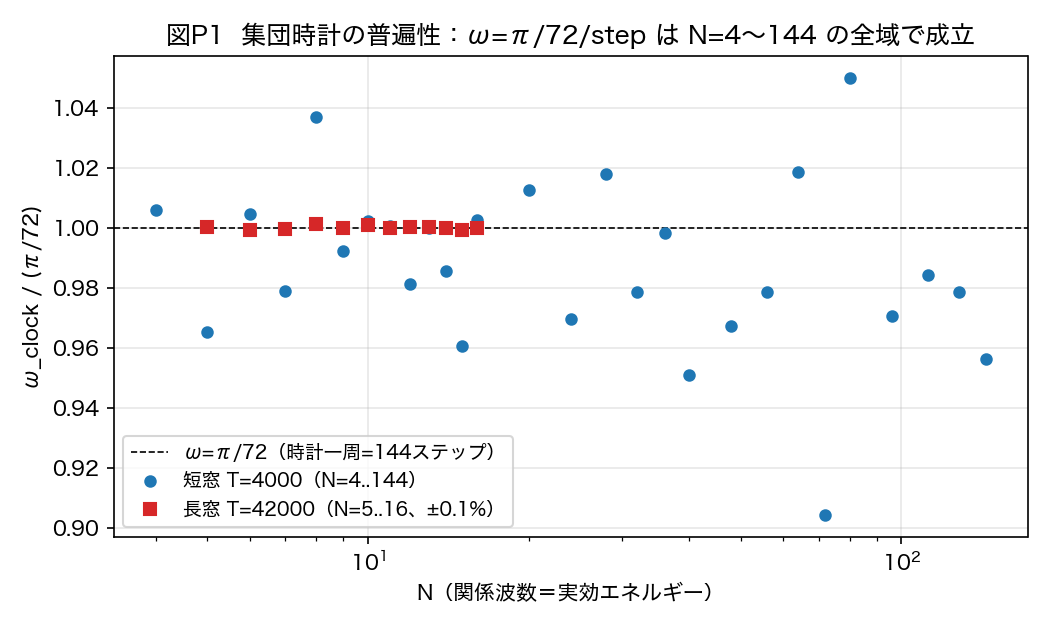
\includegraphics[keepaspectratio,alt={図P1}]{fig_p1_clock_universality_v1.png}}
\caption{図P1}
\end{figure}

\textbf{図P1}: 時計普遍性。全Nで ω/(π/72)=1。

さらに長窓の census は、低エネルギー領域（N≤16）の海で長時間定常な種が
\textbf{時計にロックした無質量基底種 ρ=1/1
ただ一つ}であることを示した（\textbar ρ−1\textbar\textless9×10⁻⁴・
質量度
10⁻¹¹）。短窓で見える質量を持つ側帯は全て有限寿命の過渡であり、時計へ
引き込まれて消える（図P2）。この反証過程（短窓の見かけの番地と質量則が長窓で
消える）は §12 に全記録した。

\begin{figure}
\centering
\pandocbounded{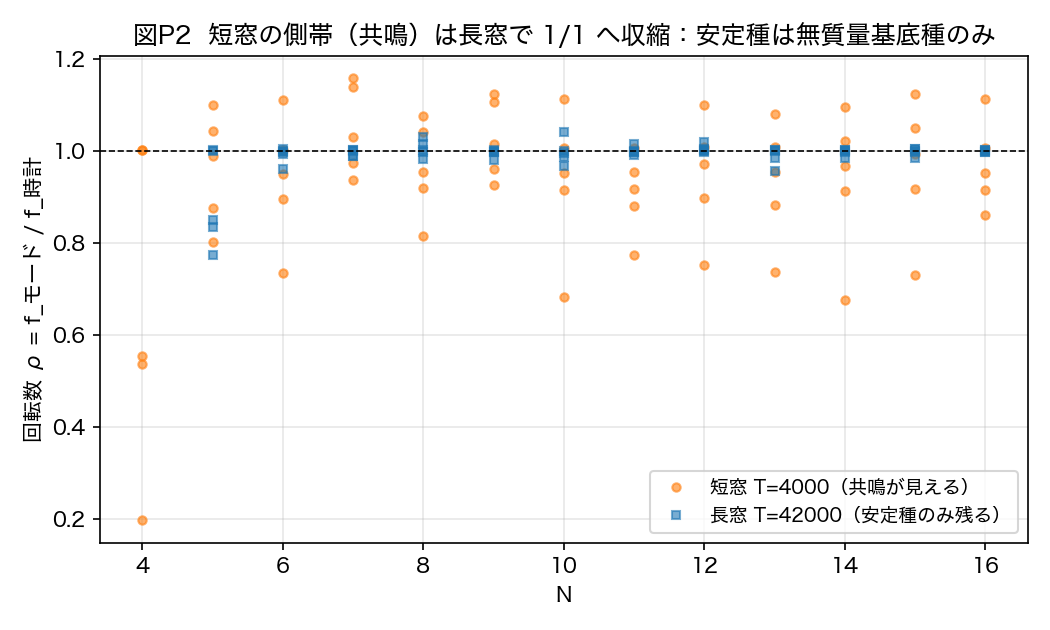
\includegraphics[keepaspectratio,alt={図P2}]{fig_p2_stable_vs_resonance_v1.png}}
\caption{図P2}
\end{figure}

\textbf{図P2}: 短窓の側帯（共鳴）は長窓で 1/1 へ収縮する。

\textbf{仮説（柱1）}: 粒子種の分類子は U\^{}n=I
の有理番地であり、土台は単一の U\^{}144
時計格子である。種は「番地（巻き数）×時計との関係」で分類される。

\subsection{4. 柱2: 電荷則------Q\_em = m/3 と閉じ込め＝mod 3
可読性}\label{ux67f12-ux96fbux8377ux5247q_em-m3-ux3068ux9589ux3058ux8fbcux3081mod-3-ux53efux8aadux6027}

\subsubsection{4.1
電荷の多値性（状態側の実測）}\label{ux96fbux8377ux306eux591aux5024ux6027ux72b6ux614bux5074ux306eux5b9fux6e2c}

帯電種（巻き
q=+1）は中性過渡より桁で長寿命（τ≈1.3×10⁴衝突・保持85\%）だが、
永続はしない。その崩壊は消失ではなく、和則 m* = 2m\_B − m\_s {[}4{]}
のウォークによる
相棒（+3）への移送である（図P3）。さらに孤立した純粋巻き数種は\textbf{任意の
m で 厳密に自己複製し}（保持率 1.000・τ 数値∞）、海なしの混合 \{+1,+3\}
すら漏れない ------\textbf{ウォークの駆動には m=0
の海が必須}である（漏れ先 \{0,−1,+2\}/\{±4\} は和則の
積と完全整合）。前論文 {[}5{]} §9.5
の「電荷が±1に安定しない」は、この海駆動 ウォークの直接の帰結である。

\begin{figure}
\centering
\pandocbounded{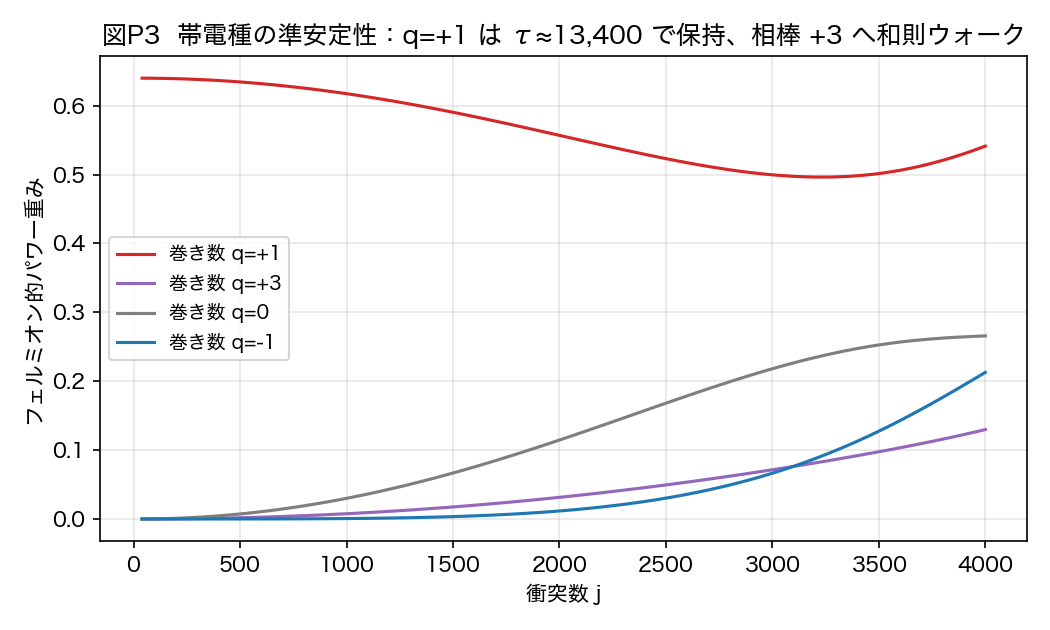
\includegraphics[keepaspectratio,alt={図P3}]{fig_p3_charged_lifetime_walk_v1.png}}
\caption{図P3}
\end{figure}

\textbf{図P3}: 帯電種の準安定性と和則ウォーク（+1→+3）。

\subsubsection{4.2
巻き数電荷の保存則は巡回である}\label{ux5dfbux304dux6570ux96fbux8377ux306eux4fddux5b58ux5247ux306fux5de1ux56deux3067ux3042ux308b}

巻き数電荷の真の保存則は整数ではなく \textbf{mod
ne（ηレジスタ位数、本系では16）の
巡回保存}である。点毎相互作用はηスペクトルの巡回畳み込みであり（連続極限では
δQ = R∮∂\_η(s²) = 0）、整数電荷 Q\_wind
の保存は帯域内状態の系にすぎない（帯電 census 構成で CV≈0
の厳密保存を実測、図P6a）。見かけの破れは倍加ウォークが Nyquist
に届いた折返しである（端パワー37\%蓄積・相関
−0.93、図P6b）。有限レジスタ 上で倍加梯子は 1→2→4→8→0 と
4歩で中性化する。

\begin{figure}
\centering
\pandocbounded{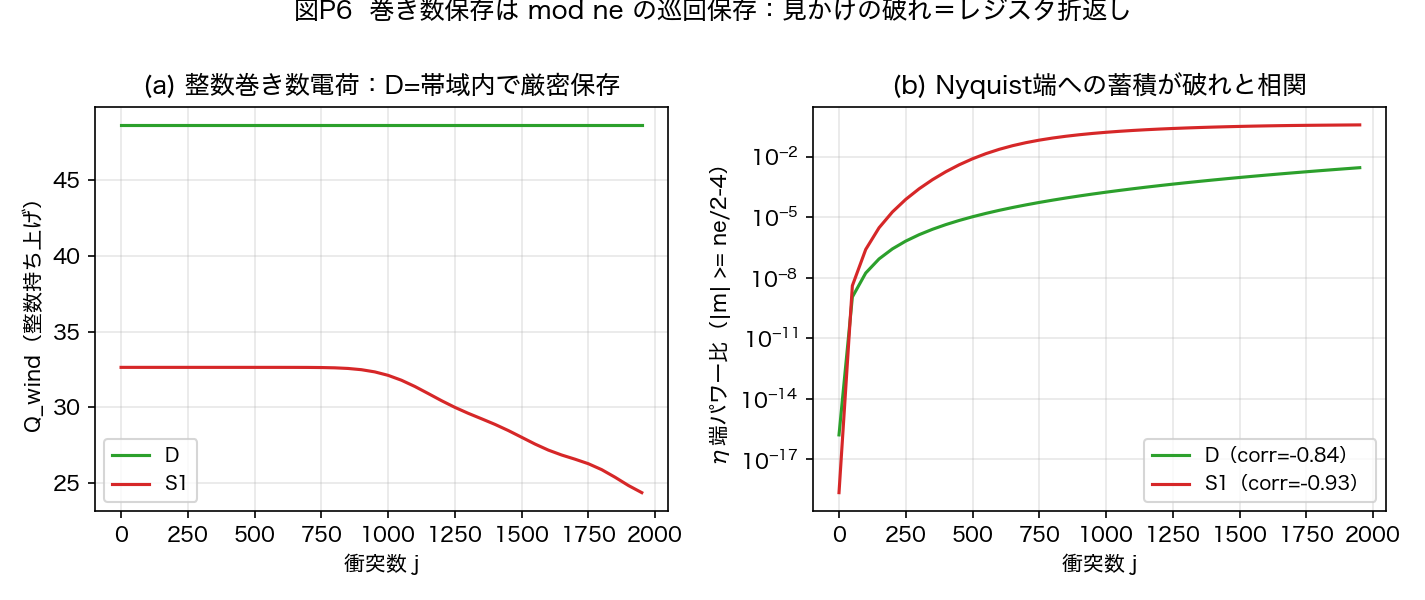
\includegraphics[keepaspectratio,alt={図P6}]{fig_p6_cyclic_conservation_v1.png}}
\caption{図P6}
\end{figure}

\textbf{図P6}: 巡回保存と Nyquist 折返し。

\subsubsection{4.3
読出し整流（読出し側の実測）}\label{ux8aadux51faux3057ux6574ux6d41ux8aadux51faux3057ux5074ux306eux5b9fux6e2c}

海駆動ウォークの全生成物（倍加・反転梯子
2\^{}b·(±1)）に対し、\textbf{観測時計 J=3 だけが 荷電内容の全てを
\textbar q\textbar=1 に読む}（集中度 1.000------+1種の宇宙でも
+2種の宇宙でも）。 J=4 は電荷を消し、J=5, 6
は多値に散らす（図P4）。代数的根拠は 2\^{}b mod 3 = ±1。
観測時計が分母3であることは、先行実測
{[}6{]}{[}7{]}------ロックのタング幅は分母3が
幅比\textgreater461で支配する------に基づく。素電荷の値そのものは有理番地
sin²(23π/124) = √(4πα)（16/10⁸ 一致）として既公開の実測 {[}6{]}
に接続する。

\begin{figure}
\centering
\pandocbounded{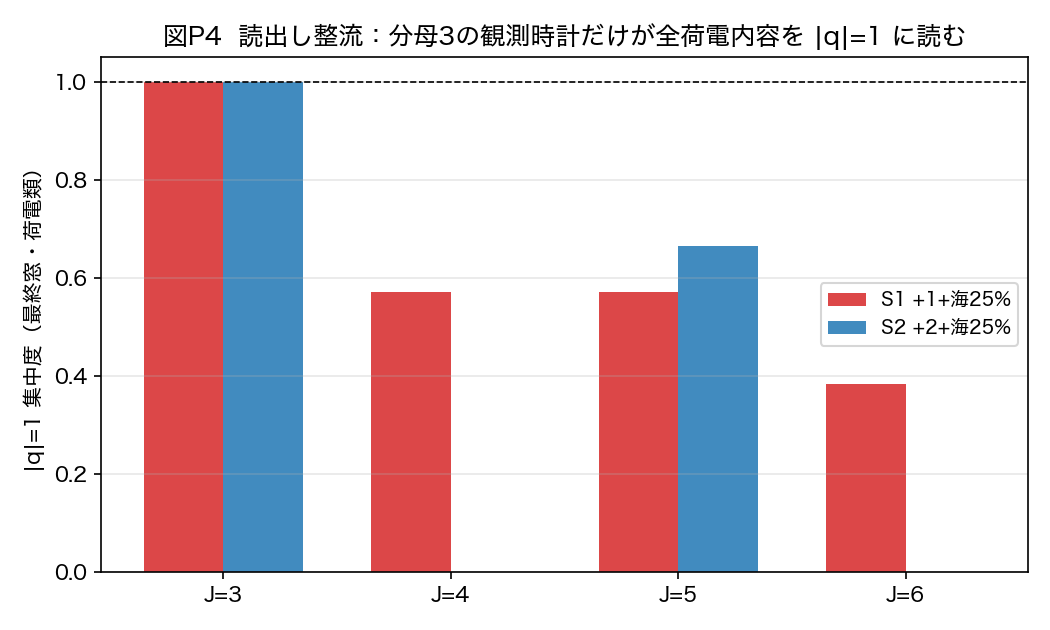
\includegraphics[keepaspectratio,alt={図P4}]{fig_p4_rectification_v1.png}}
\caption{図P4}
\end{figure}

\textbf{図P4}: 読出し整流。分母3の観測時計だけが全荷電内容を
\textbar q\textbar=1 に読む。

簿記も閉じる: 保存構成において ΔQ3 = −3ΔW が精度 7×10⁻¹⁰
で成立する（Q3=mod3で
読める正味電荷、W=mod3中性複合に隠れた電荷の帳簿）。\textbf{読める電荷は消えない------
その減少は、分母3時計に中性と読める複合への持ち込みと厳密に等しい}（図P5）。

\begin{figure}
\centering
\pandocbounded{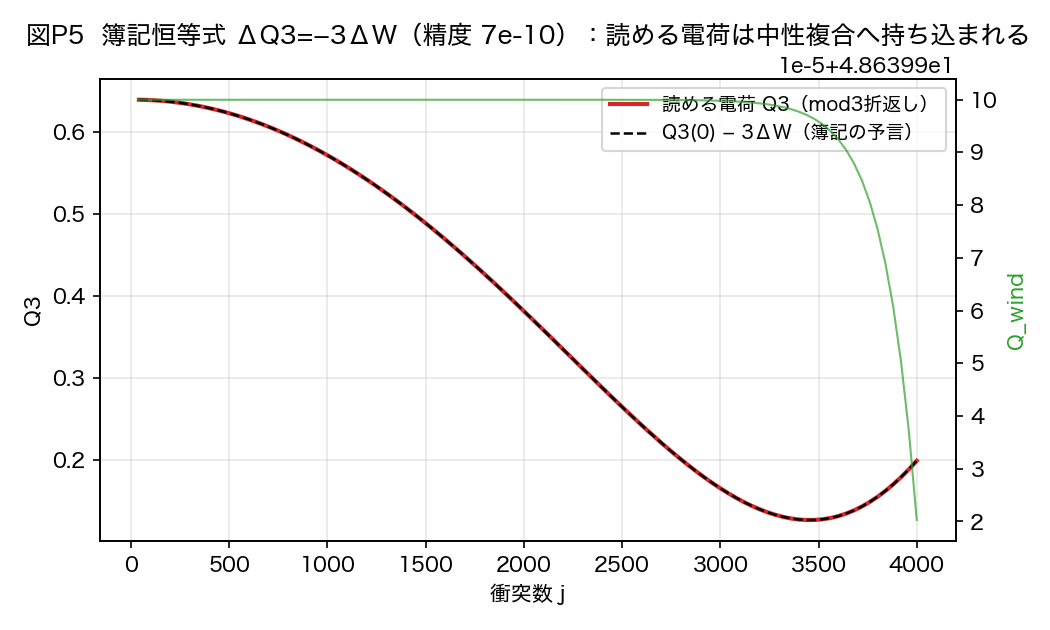
\includegraphics[keepaspectratio,alt={図P5}]{fig_p5_ledger_v1.png}}
\caption{図P5}
\end{figure}

\textbf{図P5}: 簿記恒等式 ΔQ3 = −3ΔW。

\subsubsection{4.4 仮説（柱2）: Q\_em = m/3
と閉じ込め}\label{ux4eeeux8aacux67f12-q_em-m3-ux3068ux9589ux3058ux8fbcux3081}

以上を束ねる電荷則を提案する: \textbf{電荷は Q\_em = m/3
であり、支配的観測時計（分母3） が「3生巻き＝素電荷1」と読む。} 帰結:

\begin{itemize}
\tightlist
\item
  u型 m=+2 → +2/3、d型 m=−1 → −1/3、電子 m=−3 → −1、ν m=0 → 0。
\item
  \textbf{閉じ込め＝mod 3 可読性}: 観測者の空間はη円の Z₃
  商であり、その上で一価な 種（m≡0 mod
  3）だけが自由に読出せる。クォーク（m≢0）は単独では非可読------
  \textbf{1/3電荷と閉じ込めは同一の事実の二面}であり、別々の説明を要しない。
\item
  検算: 陽子 uud = 2+2−1 = +3 → Q=+1。中性子 udd = 2−1−1 = 0 → Q=0。
  π⁺(ud̄) = 2+1 = +3 → +1。\textbf{全ハドロンの整数電荷が自動で従う。}
\end{itemize}

\textbf{閉じ込め検定（実測）}: クォーク型（m=+2）＋海は可読分率 f\_read
= 0.0000 から 出発し、ウォークが m≡0
複合（ハドロン相当）を作った分だけ可読化する
（→0.2504/4000衝突）。電子型（m=+3）＋海は f\_read = 1.0000 から出発する
（最初から自由）。\textbf{クォーク型の孤立系は4000衝突走っても f\_read =
0.0000 の
まま}------「単独のクォークは観測できない」が読出しの帰結として実現する（図P9）。

\begin{figure}
\centering
\pandocbounded{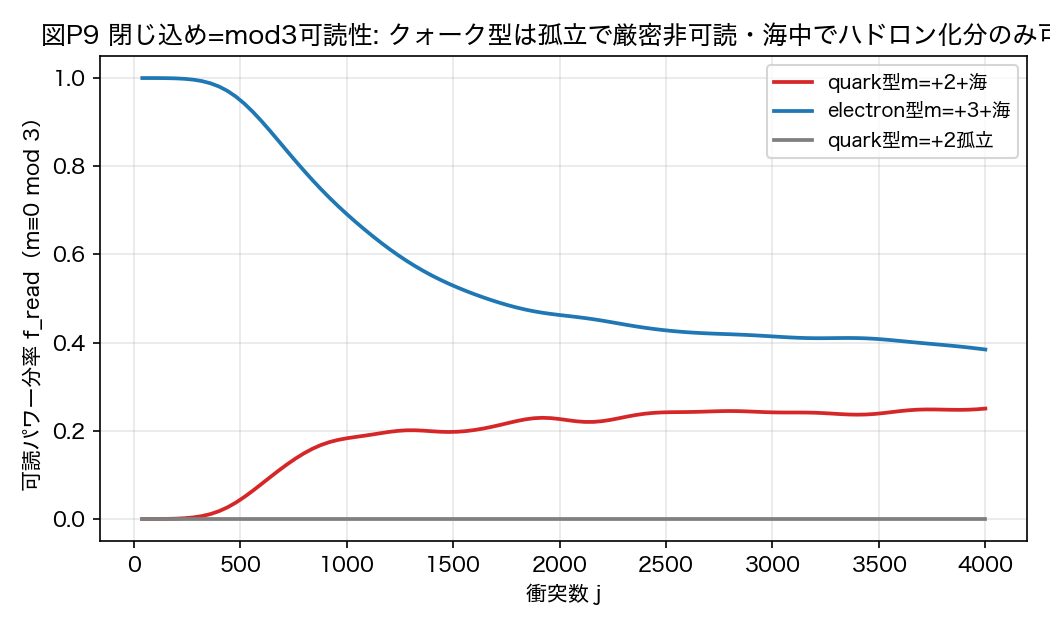
\includegraphics[keepaspectratio,alt={図P9}]{fig_p9_confinement_v1.png}}
\caption{図P9}
\end{figure}

\textbf{図P9}: 閉じ込め＝mod 3 可読性の検定。

標準理論との対応: 「自由な状態は triality 0 のみ」という SU(3) 中心 Z₃
の超選択 {[}10{]}{[}11{]} と同型の構造である。ただし標準理論では Z₃
はゲージ群の中心として力学側の 公理に入るのに対し、本仮説では mod 3
は観測時計の支配分母（実測）として
\textbf{読出し側}から出る------これが本稿の新規性の一つである（§9）。

\textbf{主張の精密化（2点）}: (i)
本節には二つの論理があり区別する------「分母3時計が
荷電ウォークを±1に整流する」は実測、「物理電荷を m/3
と同定する」は仮説である。
同定を法則に昇格させるには、電荷による\textbf{応答}------異なる m
の種の相互作用強度 Γ\_int が m/3（または
(m/3)²）に比例するか------の動力学的検定が要る（§13）。 (ii)
本稿の閉じ込めは\textbf{読出しレベルの閉じ込め}（単独非可読性）であり、標準的な
閉じ込めが含む分離エネルギーの増大・フラックス管・漸近的自由はまだ導出していない。
正確には\textbf{閉じ込めの読出し的前駆構造}であり、二つの非可読種を引き離すコストが
距離とともに増えるかの検定（§13）が動力学的閉じ込めへの昇格条件である。

\subsection{5. 柱3: 統計則------Z₂
時計被覆}\label{ux67f13-ux7d71ux8a08ux5247zux2082-ux6642ux8a08ux88abux8986}

\subsubsection{5.1
統計は空間回転に住まない（実測）}\label{ux7d71ux8a08ux306fux7a7aux9593ux56deux8ee2ux306bux4f4fux307eux306aux3044ux5b9fux6e2c}

チャネル二重項の全体回転は力学の厳密対称性であり（対照実験で全観測量が機械零で
平坦・Im(b̄a) の回転不変を解析確認）、空間回転荷は全観測モードで
ℓ=±1（校正後、 N=6, 8
で偏差±0.01以内）------半整数もℓ=2も占有モードには現れない。統計の二値性は
チャネル側にも空間側にも住んでいない。

\subsubsection{5.2
統計は時計の二重被覆に住む（実測）}\label{ux7d71ux8a08ux306fux6642ux8a08ux306eux4e8cux91cdux88abux8986ux306bux4f4fux3080ux5b9fux6e2c}

種の状態位相を観測回帰列（観測量場 s=Im(b̄a)
の自己相関ピーク列）で追うと、 \textbf{帯電種の位相は全回帰点で \{0, π\}
に厳密に量子化される}（Φ/π = ±0.999 または
+0.002・3桁精度・連続値を取らない）------状態は +1/−1
の二シートを行き来する
（図P8）。中性の非射影束は連続位相を示し、量子化の有無が種を分ける。

\begin{figure}
\centering
\pandocbounded{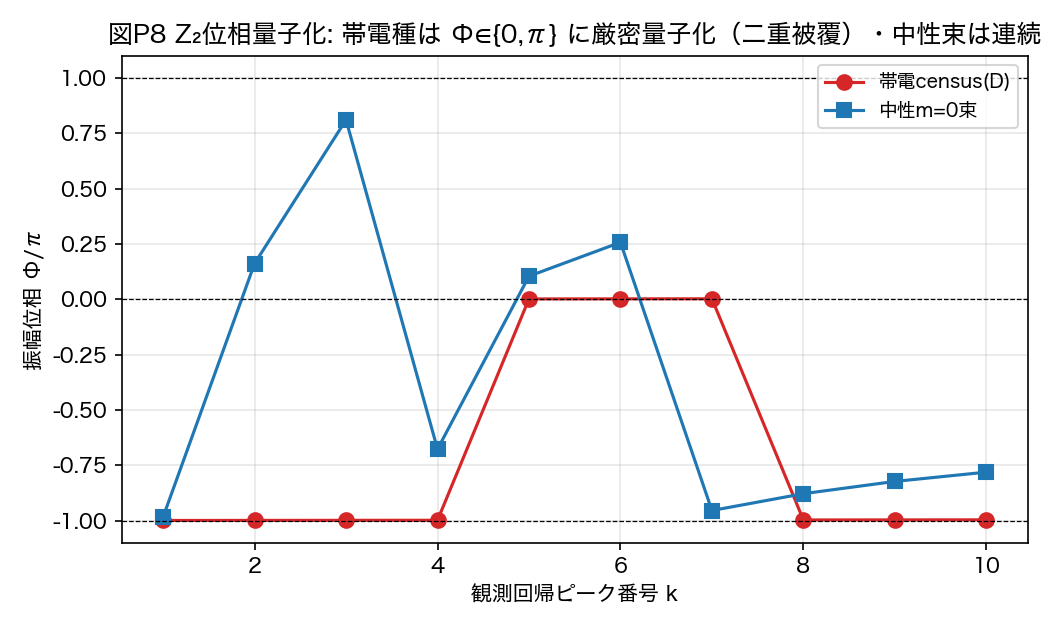
\includegraphics[keepaspectratio,alt={図P8}]{fig_p8_z2_quantization_v1.png}}
\caption{図P8}
\end{figure}

\textbf{図P8}: Z₂位相量子化。帯電種は Φ∈\{0,π\}、中性束は連続。

クロス表実験（χパリティ×巻き数 \{1,2\}
の4セル）は、\textbf{被覆度がχパリティのみに
依存し、巻き数（電荷）に依存しない}ことを示した:
フェルミオン的種（χ周波数偶
＝奇数倍音）＝被覆度2（Z₂・両シート）、ボゾン的種＝被覆度1。さらに純 m=0
の フェルミオン帯種（巻きシフト構成・η占有 (0, 1.000)）も Qz2=1.00
で被覆度2を
示した------\textbf{中性フェルミオン（ニュートリノ）の行が成立する}（図P10）。

\begin{figure}
\centering
\pandocbounded{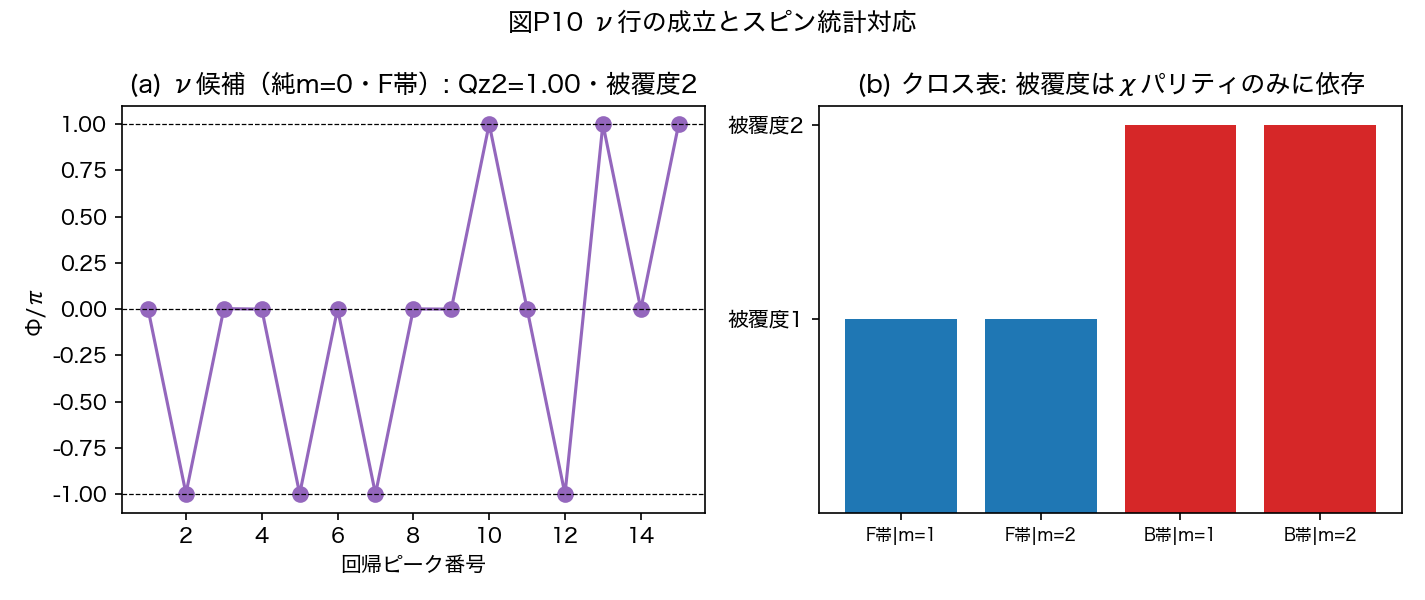
\includegraphics[keepaspectratio,alt={図P10}]{fig_p10_nu_spinstat_v1.png}}
\caption{図P10}
\end{figure}

\textbf{図P10}: ν行の成立とスピン統計対応。

\subsubsection{5.3
仮説（柱3）と先行対照}\label{ux4eeeux8aacux67f13ux3068ux5148ux884cux5bfeux7167}

\textbf{フェルミ/ボーズの区別＝時計被覆度}（1＝ボゾン的／2＝フェルミオン的）を提案
する。これは Finkelstein--Rubinstein {[}12{]}
がソリトンのスピン統計を配位空間の
二重被覆から導いた構造の対応物だが、\textbf{二重被覆の住む場所が空間（回転・交換）では
なく時計（状態周期＝観測周期×2）である}点が異なる。同構造は先行実測
{[}6{]}{[}7{]} の 位数248/観測124の忠実度（F₁₂₄側では回帰が見えず
F₂₄₈=1）と接続する。

\subsection{6. 柱4:
質量則------質量は海との関係量}\label{ux67f14-ux8ceaux91cfux5247ux8ceaux91cfux306fux6d77ux3068ux306eux95a2ux4fc2ux91cf}

\subsubsection{6.1
等価性定理（実測3件）}\label{ux7b49ux4fa1ux6027ux5b9aux7406ux5b9fux6e2c3ux4ef6}

\begin{itemize}
\tightlist
\item
  \textbf{巻きシフト等価性}: e\^{}\{imη\} は力学の厳密対称性（b̄a
  不変）であり、孤立した
  純粋番地種は全てユニタリ等価------実測でも全番地の質量²・偏極・s\_z
  が機械精度で 一致した。\textbf{質量・スピンは孤立番地の属性ではない。}
\item
  \textbf{約数類定理}: 海中では性質が分化するが、\textbf{約数類 gcd(m,
  16) までしか分化 しない}（奇数 \{1,3,5,7\} の質量²が5桁一致・\{2,6\}
  一致・\{4\} 独自、図P7）。 理由は厳密: Z₁₆ の単元自己同型 m→um
  は海（m=0）を固定するため、海結合は
  単元番地を原理的に区別できない。帰結: \textbf{±1 と ±5, ±7
  の区別は力学に存在せず、 mod3
  読出しだけが単元類を破る}------柱2（読出し整流）の独立な裏づけ。
\item
  \textbf{χ帯平行移動対称性}: 同一巻き種を χ帯
  (10,12,14)/(30,32,34)/(50,52,54) に
  置いても質量²は5桁一致------帯の位置も種を分化させない（§10 弱点1）。
\end{itemize}

\begin{figure}
\centering
\pandocbounded{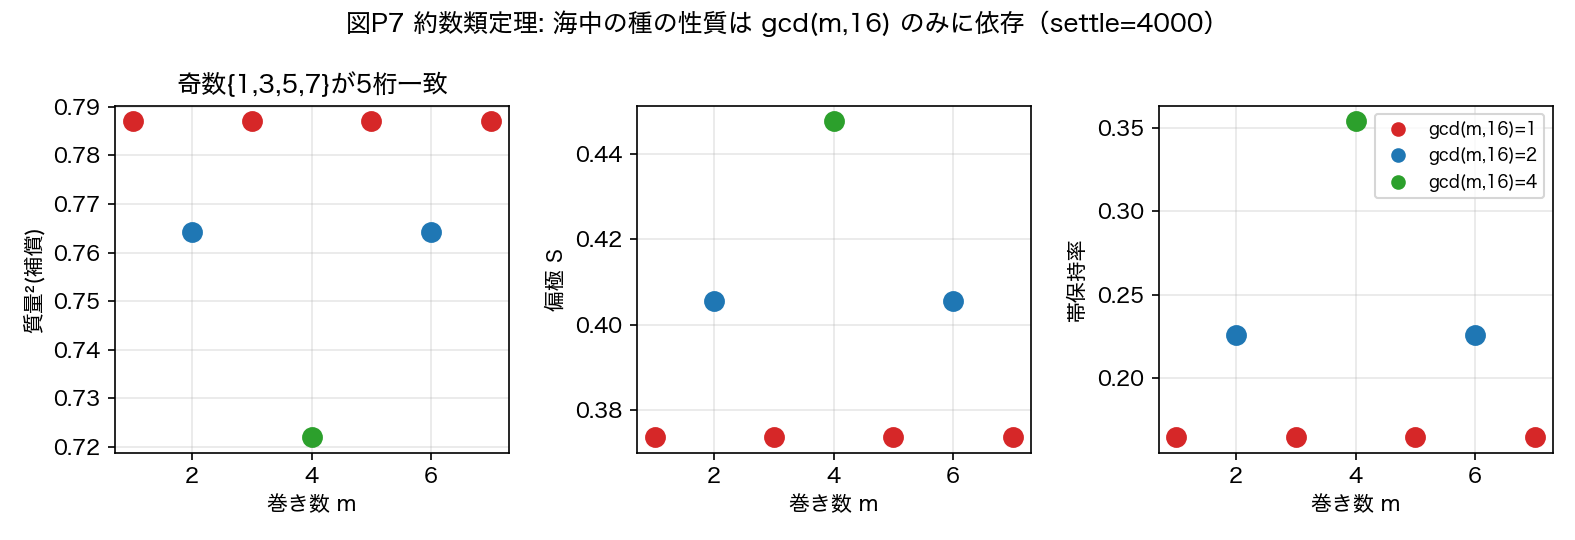
\includegraphics[keepaspectratio,alt={図P7}]{fig_p7_divisor_class_v1.png}}
\caption{図P7}
\end{figure}

\textbf{図P7}: 約数類定理。海中の性質は gcd(m,16) のみに依存する。

\subsubsection{6.2 仮説（柱4）}\label{ux4eeeux8aacux67f14}

\textbf{質量は海（真空）との関係量である。}
時計にロックした種（ρ=1/1）だけが無質量で
安定（光子的基底種・質量度10⁻¹¹実測）、時計から離れた内容は共鳴として質量を
持ち、海が種の個性（寿命・偏極・質量）を約数類の水準で分化させる。真空＝海を
粒子の性質の共同決定者とする視点は、創発ゲージ・創発フェルミオンの系譜
{[}13{]}（string-net凝縮・超流動³He）と共鳴するが、本稿は性質の海依存を等価性定理と
いう形で実測した点が異なる。

\subsection{7. 柱5:
波の周期表------二枚看板と62種割当}\label{ux67f15-ux6ce2ux306eux5468ux671fux8868ux4e8cux679aux770bux677fux306862ux7a2eux5272ux5f53}

\subsubsection{7.1 二枚看板}\label{ux4e8cux679aux770bux677f}

\begin{itemize}
\tightlist
\item
  \textbf{表A（孤立安定元素表）}: U\^{}144
  時計格子上の純粋番地種。全て自己複製で安定 （実測）。代数的分類子:
  読める電荷（mod3）・倍加軌道・中性化歩数・ηパリティ。
  第二のパリティ構造:
  奇数番地は倍加中性化に最大限（4歩）抵抗し、偶数は速く
  落ちる（±4は2歩、+8は1歩）。
\item
  \textbf{表B（海中寿命表）}:
  海結合が種を淘汰する------帯電で長寿命（τ\textasciitilde10⁴）・中性
  過渡で短寿命（τ\textasciitilde10²⁻³）・複合で中性化。\textbf{実観測される「粒子」はこの準安定
  階層である。}
\end{itemize}

\textbf{原始周期表（模型固有・実測に基づく主表）}:
標準模型の粒子名を使わずに、
本稿の分類子だけで書いた表を先に置く。標準模型への割当（§7.2）はこの表の上の
仮説である。

{\def\LTcaptype{none} % do not increment counter
\begin{longtable}[]{@{}
  >{\raggedright\arraybackslash}p{(\linewidth - 12\tabcolsep) * \real{0.1429}}
  >{\raggedright\arraybackslash}p{(\linewidth - 12\tabcolsep) * \real{0.1429}}
  >{\raggedright\arraybackslash}p{(\linewidth - 12\tabcolsep) * \real{0.1429}}
  >{\raggedright\arraybackslash}p{(\linewidth - 12\tabcolsep) * \real{0.1429}}
  >{\raggedright\arraybackslash}p{(\linewidth - 12\tabcolsep) * \real{0.1429}}
  >{\raggedright\arraybackslash}p{(\linewidth - 12\tabcolsep) * \real{0.1429}}
  >{\raggedright\arraybackslash}p{(\linewidth - 12\tabcolsep) * \real{0.1429}}@{}}
\toprule\noalign{}
\begin{minipage}[b]{\linewidth}\raggedright
生巻き類
\end{minipage} & \begin{minipage}[b]{\linewidth}\raggedright
mod3可読
\end{minipage} & \begin{minipage}[b]{\linewidth}\raggedright
中性化歩数
\end{minipage} & \begin{minipage}[b]{\linewidth}\raggedright
時計被覆（F帯/B帯）
\end{minipage} & \begin{minipage}[b]{\linewidth}\raggedright
海中質量²（約数類）
\end{minipage} & \begin{minipage}[b]{\linewidth}\raggedright
孤立安定性
\end{minipage} & \begin{minipage}[b]{\linewidth}\raggedright
海中寿命
\end{minipage} \\
\midrule\noalign{}
\endhead
\bottomrule\noalign{}
\endlastfoot
m=0 & 0（自由・中性） & 0 & 2 / 1 & ---（海・基底種） & 安定 &
基底種は安定 \\
奇数（単元）\{±1,±3,±5,±7\} & ±1 or 0 & 4（最大） & 2 / 1 &
0.787（5桁一致） & 厳密安定 & τ\textasciitilde10⁴（帯電） \\
\{±2,±6\} & ∓1 or 0 & 3 & 2 / 1 & 0.764 & 厳密安定 & 保持率0.226 \\
\{±4\} & ±1 & 2 & 2 / 1 & 0.722 & 厳密安定 & 保持率0.354（最長） \\
\{+8\} & −1 & 1（最短） & --- & 未測 & --- & 未測 \\
\end{longtable}
}

被覆度は生巻き類でなくχパリティで決まる（クロス表実測）ため独立列である。

\subsubsection{7.2
標準模型62種の割当案}\label{ux6a19ux6e96ux6a21ux578b62ux7a2eux306eux5272ux5f53ux6848}

確度記号:
\textbf{E}=実測錨（本稿または既公開の実測が直接支える）／\textbf{S}=構造対応
（機構は一致するが定量未検証）／\textbf{H}=仮説（今後の検証対象）。

{\def\LTcaptype{none} % do not increment counter
\begin{longtable}[]{@{}
  >{\raggedright\arraybackslash}p{(\linewidth - 10\tabcolsep) * \real{0.1667}}
  >{\raggedright\arraybackslash}p{(\linewidth - 10\tabcolsep) * \real{0.1667}}
  >{\raggedright\arraybackslash}p{(\linewidth - 10\tabcolsep) * \real{0.1667}}
  >{\raggedright\arraybackslash}p{(\linewidth - 10\tabcolsep) * \real{0.1667}}
  >{\raggedright\arraybackslash}p{(\linewidth - 10\tabcolsep) * \real{0.1667}}
  >{\raggedright\arraybackslash}p{(\linewidth - 10\tabcolsep) * \real{0.1667}}@{}}
\toprule\noalign{}
\begin{minipage}[b]{\linewidth}\raggedright
粒子
\end{minipage} & \begin{minipage}[b]{\linewidth}\raggedright
状態数
\end{minipage} & \begin{minipage}[b]{\linewidth}\raggedright
巻き m（Q\_em=m/3）
\end{minipage} & \begin{minipage}[b]{\linewidth}\raggedright
被覆
\end{minipage} & \begin{minipage}[b]{\linewidth}\raggedright
確度
\end{minipage} & \begin{minipage}[b]{\linewidth}\raggedright
摘要
\end{minipage} \\
\midrule\noalign{}
\endhead
\bottomrule\noalign{}
\endlastfoot
u, c, t & 18 & +2（+2/3） & 2 & \textbf{E} &
m≢0→閉じ込め（図P9実測）。色=mod3非可読の生巻き残差（簿記W） \\
d, s, b & 18 & −1（−1/3） & 2 & \textbf{E} & 同上 \\
e, μ, τ & 6 & −3（−1） & 2 & \textbf{E} & 自由（m≡0）。素電荷番地
sin²(23π/124) {[}6{]} \\
ν ×3 & 6 & 0（0） & 2 & \textbf{E} &
中性フェルミオン（§5.2実測で成立） \\
γ & 1 & 0 & 1 & \textbf{E} & 基底種 ρ=1/1（無質量・安定・実測） \\
g & 8 & 色対（mod3中性・生巻き非零） & 1 & S &
色非一重項→単独非可読=閉じ込め。8重項の生成は未導出 \\
W±, Z & 3 & ±3, 0 & 1 & S &
t巻き（自前時計の離調）→有質量（引き込み実測と整合・力学未検証） \\
H & 1 & 0 & 1 & S & 海（凝縮体）の集団モード。ℓ=0 \\
G & 1 & 0 & 1 & H & ℓ=1量子2個の複合のみ（§8.4予言）。ℓ=±2 \\
（世代軸） & --- & --- & --- & H & 3世代の分化軸は未同定（§10） \\
\end{longtable}
}

計 \textbf{62種}（クォーク36＋レプトン12＋g8＋γ＋W2＋Z＋H＋G）。反粒子は
m→−m （電荷共役＝η反転・対生成は実測 {[}3{]}）。世代 g=1,2,3
の割当軸は未解決（§10）。
各行の確度（実測錨／構造対応／要検定仮説）は添付の周期表第0.4版に明示した。

\subsubsection{7.3
二つの有限構造の関係（開いた構造問題）}\label{ux4e8cux3064ux306eux6709ux9650ux69cbux9020ux306eux95a2ux4fc2ux958bux3044ux305fux69cbux9020ux554fux984c}

本稿には二つの有限構造が実測されている: 普遍時計
U\^{}144（§3）と巻きレジスタ Z₁₆（§4.2）。因数構造は 144 = 2⁴·3²、16 =
2⁴、144/16 = 9 = 3² であり、
本稿の分類子はこの因数に対応する------\textbf{2＝統計被覆（§5）、3＝電荷可読性（§4）、
16＝生巻き巡回（§4.2）}。この一致が偶然か、更新則から両方が従う共鳴構造
（時計位数×内部巻き位数の共鳴分類）かは、本稿最大の開いた構造問題であり、
数合わせではなく\textbf{作用素の回帰構造として}検定すべき課題として §13
に登録する。 定式化:
各読出し操作を同一の作用素表現に持ち込み、部分空間ごとの位数
ord(U\textbar\_\{H\_i\})
を測る------本当の周期律は「同一作用素が異なる読出し部分空間で持つ
位数」の族である可能性がある。「周期表」の本当の周期律はおそらくここに住む。

\subsection{8.
説明力------既存課題への接続}\label{ux8aacux660eux529bux65e2ux5b58ux8ab2ux984cux3078ux306eux63a5ux7d9a}

\subsubsection{8.1
前論文の未解決課題「電荷±1非安定」の解決}\label{ux524dux8ad6ux6587ux306eux672aux89e3ux6c7aux8ab2ux984cux96fbux83771ux975eux5b89ux5b9aux306eux89e3ux6c7a}

前論文 {[}5{]} §9.5
は「電荷（巻き数）は±1に安定せず複数の値に分布する」を未解決
課題として明記した。本仮説の下でこれは矛盾ではない:
\textbf{状態側}では海駆動ウォーク
（実測・§4.1）が巻き数を分散させ続ける。\textbf{読出し側}では分母3の観測時計がその
全生成物を \textbar q\textbar=1
に折り返して読む（実測・§4.3）。「電荷の多値性」と「素電荷の
普遍性」は矛盾なく同居する------未解決課題が仮説の予言に転じる。

\subsubsection{8.2
クォークの1/3電荷問題}\label{ux30afux30a9ux30fcux30afux306e13ux96fbux8377ux554fux984c}

Q\_em = m/3
の下で、分数電荷（なぜ1/3か）と閉じ込め（なぜ単独で見えないか）は mod 3
可読性という単一機構である（§4.4・実測図P9）。

\subsubsection{8.3 反物質}\label{ux53cdux7269ux8cea}

電荷共役 m→−m はスペクトルの対称であり、対生成はウォークの必然である
（既公開実測 {[}3{]}）。

\subsubsection{8.4 重力の弱さ}\label{ux91cdux529bux306eux5f31ux3055}

凝縮体の回転生成子スペクトルに ℓ=2 の線形枠は存在しない（校正比最大
1.000 厳密・
実測）。スピン2はℓ=1量子2個の\textbf{複合}としてのみ存在でき、実際に読出し二乗の
スペクトルには 2ω の四重極線が全Nでコヒーレントに立つ（比
2±6\%）。複合である ことの直接の帰結として結合は二乗抑制 α\_G=(m/M)²
{[}15{]} を受ける------\textbf{重力が弱い
理由と検証が難しい理由は同一構造}である。これは重力振幅＝ゲージ振幅²
（double copy {[}16{]}）と同型の構造の、状態空間側からの出現である。

\subsection{9.
先行研究との関係と新規性の限定}\label{ux5148ux884cux7814ux7a76ux3068ux306eux95a2ux4fc2ux3068ux65b0ux898fux6027ux306eux9650ux5b9a}

本仮説の部品にはそれぞれ強い先行系譜がある: 巻き数＝荷（Skyrme
{[}17{]}・ Kaluza--Klein {[}18{]}）、mod3 閉じ込め（triality
{[}10{]}{[}11{]}）、統計の二重被覆 （Finkelstein--Rubinstein
{[}12{]}）、真空＝海（Wen・Volovik {[}13{]}）、重力＝二乗 （KLT/BCJ
{[}16{]}）、全種割当の企図（八道説 {[}9{]}・プレオン {[}14{]}）。
\textbf{本稿は部品の新規性を主張しない。} 新規性は次の3点に限定する:

\begin{enumerate}
\def\labelenumi{\arabic{enumi}.}
\tightlist
\item
  これらの部品が、粒子概念を仮定しない\textbf{単一の無名力学の実測}として同時に
  出ること（合流）。
\item
  電荷単位・閉じ込め・素電荷一意性が、力学側の公理（ゲージ群の中心）ではなく
  \textbf{観測時計の約数構造（読出し側）}から出るという対応物の提示。
\item
  統計の二重被覆が空間（配位空間の回転）ではなく\textbf{時計}（状態周期＝観測周期×2）
  に住むという実測。
\end{enumerate}

\subsection{10.
仮説の弱点と未検証部分（正直な登録）}\label{ux4eeeux8aacux306eux5f31ux70b9ux3068ux672aux691cux8a3cux90e8ux5206ux6b63ux76f4ux306aux767bux9332}

\begin{enumerate}
\def\labelenumi{\arabic{enumi}.}
\tightlist
\item
  \textbf{世代の起源は未解決}:
  世代＝χ帯位置の素朴仮説は反証済み（χ帯平行移動
  対称性・§6.1）。帯比・結晶学的位数 \{3,4,6\}・複合階層が残る候補。
\item
  \textbf{W/Z行}:
  低エネルギー実験室（N≤16・小さな海）では直接生成不可（レジスタ端
  即崩壊・構造的）。有効接触頂点の 1/δ²
  スケーリング検定（Fermi理論の道）を 指定済み・未実施。
\item
  \textbf{グラビトン行}:
  四重極2ω線は全Nで実在するが、事前基準（\textbar 比−2\textbar\textless0.02）は
  1/3のみ通過------読出し枠の較正が未了。
\item
  \textbf{レジスタ位数 ne=16 依存性}: 表Aの詳細（中性化歩数等）は ne
  の関数である。 ne
  可変系での再検が必要（「周期表の周期はレジスタ位数の関数」という検証可能
  予言でもある）。
\item
  \textbf{Q\_em = m/3 と透過率電荷 √(4πα) {[}6{]}{[}19{]}
  の二読出しの統一は未完}------素電荷の
  「単位」（3巻き）と「値」（0.302822）の関係は次論文の課題。
\item
  海構成の一部（人工射影海）は保存クラス外と判明済み（Nyquist折返し・§4.2）。
  該当実験の定量は保留付きで扱い、定性結論は保存クラス内の系列で整合確認した。
\end{enumerate}

\subsection{11. 反証条件}\label{ux53cdux8a3cux6761ux4ef6}

\begin{enumerate}
\def\labelenumi{\arabic{enumi}.}
\tightlist
\item
  分母3以外の観測時計が、同一の荷電ウォーク生成物の集合全体を一意の素電荷
  単位に整流する例が構成されれば、柱2は棄却される。
\item
  同じ凝縮相・同じ更新則・同じ整定基準の長窓極限で、ω が π/72
  から系統的に 逸脱する系列が得られれば、柱1は棄却される。
\item
  被覆度がχパリティと独立に変わる種が構成されれば、柱3は棄却される。
\item
  海なしで種の性質（質量・寿命・偏極）が分化する実測が出れば、柱4は棄却される。
\item
  m≢0 (mod 3)
  の種が単独で可読になる構成が見つかれば、閉じ込め則は棄却される。
\end{enumerate}

\subsection{12.
反証と修正の記録（13件・要約）}\label{ux53cdux8a3cux3068ux4feeux6b63ux306eux8a18ux933213ux4ef6ux8981ux7d04}

本研究の過程で反証された仮説と計器を全て記録する: (1)
短窓の側帯番地は安定種では なく過渡（長窓で消滅）。(2)
質量＝離調²則は過渡上の見かけの関係。(3) ±1不動点
一意性の素朴形（任意の純粋mが不動点であり一意性は出ない）。(4)
質量-幅相関は 不成立（r=−0.07）。(5)
海構成規約（χ解析射影）仮説は不成立------保存の破れの正体は
Nyquist折返し（§4.2）。(6)
escape率による±1一意性は約数類定理により原理的に 判定不能と判明。(7)
SU(2)回帰角判別の運動学版は全状態でスピノル的（自明）。 (8)
被覆度の単点判定は位相の偶然のπ近傍を拾う（回帰列判定に較正）。 (9)
グラビトンℓ=2の線形枠は不在（複合へ再解釈）。(10) 世代＝χ帯位置は反証。
(11) W/Z離調注入の帯シフト法は失敗（実効線形分散）。(12)
ν構成の射影法は失敗 （束の毛m=+1が原因・シフト法で解決）。(13)
過去の射影海は増幅数値残差
（m=0場として正当・定性不変・記録）。各件の詳細は添付の分析ノートにある。

\subsection{13.
統一動力学への要件引き継ぎ（次論文の仕様）}\label{ux7d71ux4e00ux52d5ux529bux5b66ux3078ux306eux8981ux4ef6ux5f15ux304dux7d99ux304eux6b21ux8ad6ux6587ux306eux4ed5ux69d8}

本稿の分類仮説を力学レベルで検証するには、現在二系に分かれている力学を単一の
\textbf{万能相互作用関数}に統一し、62種がそのスペクトルとして生成・崩壊・相互作用する
ことを示す必要がある。本稿の実測は、その関数が満たすべき要件を確定する:

\begin{enumerate}
\def\labelenumi{\arabic{enumi}.}
\tightlist
\item
  \textbf{無名性}:
  波の形だけを入力とし、種ごとの場合分けを持たない（IF文なし）。
\item
  \textbf{全チャネル同時}:
  電磁（巻き交換）・弱（時計離調）・強（mod3非可読の生巻き
  残差）・重力（二次モーメント結合）が、別々の項でなく同一演算の異なる読出しと
  して出ること。三平面（xy=スピン／zR=質量／tQ=電荷）{[}20{]}
  を同時に駆動する。
\item
  \textbf{保存則の自動成立}:
  巡回巻き保存（§4.2）・閉塞保存・ノルム保存を設計でなく
  演算構造から保つ。
\item
  \textbf{普遍時計の再現}: ω=π/72 の U\^{}144
  時計格子（§3）がスペクトルとして出る。
\item
  \textbf{選択則の創発}: 和則
  m*=2m\_B−m\_s・倍加反転梯子・Z₂位相量子化・約数類構造が
  手置きなしに出る。
\item
  \textbf{厳密計算可能性}: 無名性⇒状態サイズ線形の計算構造 {[}4{]}
  を保つ（閉形式または 整数厳密）。
\item
  \textbf{二系の特殊化}: 二体閉形式解 {[}3{]} と N体関係波力学 {[}2{]}
  が、その関数の 制限・極限として再導出される。
\item
  \textbf{反証形}:
  62種割当（§7.2）のいずれかがスペクトルに現れなければ、本稿の
  周期表仮説は該当行ごとに棄却される。
\end{enumerate}

\subsubsection{13.2
検証プログラム（最優先4件）}\label{ux691cux8a3cux30d7ux30edux30b0ux30e9ux30e0ux6700ux512aux51484ux4ef6}

万能関数の構築と並行して、本稿の仮説を直接強化・反証しうる実験を優先順に登録する:

\begin{enumerate}
\def\labelenumi{\arabic{enumi}.}
\tightlist
\item
  \textbf{分母3の力学的導出と電荷応答}:
  観測時計の分母3支配は現在ロック実測 {[}20{]} に
  基づく。この力学で分母3の Arnold tongue が最大になる理由の解析的導出が
  得られれば、Q\_em = m/3
  の「3」は経験的選択から力学的必然へ進む。あわせて、 二種 (m₁, m₂)
  の交換量・位相変化が積 m₁m₂/9 に比例するか（クーロン型の
  電荷積検定）を測る------通れば m/3
  は帳簿から相互作用に現れる物理電荷へ昇格する。
\item
  \textbf{時計被覆度と交換符号の同一実験（万能関数の構築に先行して実施すべき決定実験）}:
  被覆度2 ⟺ 二つの同種の交換符号 −1 を同一実験で結ぶ。交換操作 E
  と時計一周 操作 T が状態空間上で同じ二重被覆の非自明類に属する（E ≃
  T、E²=T²=I）ことが
  示されれば、半整数的帰還・交換符号・排他性・時計被覆度が単一の Z₂
  に縮約され、 柱3は「統計に似ている」から「統計構造の再構成」へ進む。
\item
  \textbf{レジスタ位数可変の周期表変形則}: ne = 12, 18, 24, 32, \ldots{}
  で約数類・ 中性化歩数・可読性・被覆構造が gcd(m, ne)／Div(ne)
  に追随するかを測る。
  追随すれば約数類定理が一般化され、しなければ16固有の隠れ構造がある。
\item
  \textbf{盲検予言}:
  標準模型の粒子名を使わず、模型だけから未占有番地・寿命順位・
  電荷・被覆度・崩壊先を予言し、事後に既知粒子表と照合する------八道説の
  Ω⁻ 型の 決定力を持つ検定形式。
\end{enumerate}

\subsection{14. 再現性}\label{ux518dux73feux6027}

全実験は決定論的スクリプト（28本）として本稿と同じフォルダに公開する。
対応表（実験一覧\_v1.md）にスクリプト↔結果JSON（25点）↔図（10枚）↔主張の
完全対応を示した。当初対話的に実行された3件は正式スクリプト化し、保存結果との
再現一致を機械確認済みである。判定基準は各スクリプト冒頭に実行前に固定して
記録した。

\subsection{引用文献}\label{ux5f15ux7528ux6587ux732e}

\textbf{自己引用（力学と実測の出所）} {[}1{]} 木原範昭,
思考実験「R軸について」, Zenodo (2026). doi:10.5281/zenodo.19902677
{[}2{]} 木原範昭, 二段階seed除去による準安定相の因果分離（第8論文）,
Zenodo (2026). doi:10.5281/zenodo.21614402 {[}3{]} 木原範昭,
フェルミオン的構造の生成------万能非弾性写像, Zenodo (2026).
doi:10.5281/zenodo.21808091 {[}4{]} 木原範昭,
インフレーションの終わり方が物質生成の始まり方である（多体接続）, Zenodo
(2026). doi:10.5281/zenodo.21809814 {[}5{]} 木原範昭,
空間軸3軸と固有時間の創生, Zenodo (2026). doi:10.5281/zenodo.21816651
{[}6{]} 木原範昭,
無名二チャネル閉鎖波系における数え上げ読出し（三部作B）, Zenodo (2026).
doi:10.5281/zenodo.21763997 {[}7{]} 木原範昭,
フェルミオンの生成構造（第9論文）, Zenodo (2026).
doi:10.5281/zenodo.21766706 {[}15{]} 木原範昭,
実在中心の読み直し------導出置換編, Zenodo (2026).
doi:10.5281/zenodo.21765367 {[}19{]} 木原範昭,
無名二チャネル閉鎖波系における二文法分解（三部作A）, Zenodo (2026).
doi:10.5281/zenodo.21763995 {[}20{]} 木原範昭,
無名二チャネル閉鎖波系におけるロック動力学（三部作C）, Zenodo (2026).
doi:10.5281/zenodo.21763999

\textbf{外部引用} {[}8{]} W. Thomson (Lord Kelvin), ``On Vortex Atoms,''
Proc. Roy. Soc. Edinburgh 6, 94 (1867). {[}9{]} M. Gell-Mann, ``The
Eightfold Way,'' Caltech Report CTSL-20 (1961); M. Gell-Mann and Y.
Ne'eman, The Eightfold Way (Benjamin, 1964). {[}10{]} K. G. Wilson,
``Confinement of quarks,'' Phys. Rev.~D 10, 2445 (1974). {[}11{]} G. 't
Hooft, ``On the phase transition towards permanent quark confinement,''
Nucl. Phys. B 138, 1 (1978). {[}12{]} D. Finkelstein and J. Rubinstein,
``Connection between spin, statistics, and kinks,'' J. Math. Phys. 9,
1762 (1968). {[}13{]} M. A. Levin and X.-G. Wen, ``String-net
condensation,'' Phys. Rev.~B 71, 045110 (2005); G. E. Volovik, The
Universe in a Helium Droplet (Oxford, 2003). {[}14{]} H. Harari, ``A
schematic model of quarks and leptons,'' Phys. Lett. B 86, 83 (1979); M.
A. Shupe, Phys. Lett. B 86, 87 (1979). {[}16{]} Z. Bern, J. J. M.
Carrasco, and H. Johansson, ``Perturbative quantum gravity as a double
copy of gauge theory,'' Phys. Rev.~Lett. 105, 061602 (2010); H. Kawai,
D. C. Lewellen, and S. H. H. Tye, Nucl. Phys. B 269, 1 (1986). {[}17{]}
T. H. R. Skyrme, ``A unified field theory of mesons and baryons,'' Nucl.
Phys. 31, 556 (1962). {[}18{]} T. Kaluza, Sitzungsber. Preuss. Akad.
Wiss. (1921) 966; O. Klein, Z. Phys. 37, 895 (1926). 補足: S. Coleman,
``Quantum sine-Gordon equation as the massive Thirring model,'' Phys.
Rev.~D 11, 2088 (1975) はボゾン化系譜の代表として {[}7{]}
経由で参照する。

\end{document}
